\documentclass[12pt]{article}

\usepackage{fullpage}
\usepackage{mathtools}
\usepackage{tikz}
\usepackage{caption}
\usepackage{subcaption}

\usepackage{csquotes}
\usepackage[backend=bibtex]{biblatex}
\addbibresource{node.dating}

\newcommand{\code}[1]{\emph{#1}}

\title{node.dating: methodology}

\author{Bradley R. Jones and Art F. Y. Poon}

\begin{document}
	\maketitle
	
	\section{General algorithm}	
		\code{node.dating} uses a tip to root maximum likelihood approach, based on \cite{Felsenstein81, TipDates}, to estimate the dates of the internal nodes of a phylogenetic tree given a rooted phylogentic tree with branch length in number of molecular substitutions per base and dated tips.
		
		The mutation rate, $\mu$ of the tree is estimated by estimating the parameter $\mu$ in the linear model:
		\[\mathbf{D}_n = \frac{1}{\mu}\mathbf{t}_n + a,\]
		where $\mathbf{t}_n$ is the date of the tip, $n$, of the phylogenetic tree, $\mathbf{D}_n$ is the distance of $n$ from the root and $a$ and $\mu$ are estimated parameters.
		The mutation rate can optionally be provided.
		
		Starting from the nodes furthest from the root (disregarding edge length), the date, $t^*$, of each node $n$ is chosen to maximize the product of the likelihoods, $\mathcal{L}_e(t^* - t_c)$, of its child edges (See Figure  \ref{fig:init}). This is done either using calculus if the tree is binary or the \code{optimize} function of R if the tree is not binary.
		
		\begin{figure}[h]
			\centering
			\begin{subfigure}{.3\textwidth}
			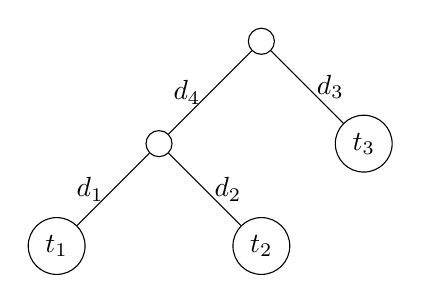
\begin{tikzpicture}[scale=1.3]
				\path (-2, -2) node[draw, circle] (n1){$t_1$}
				(0, -2) node[draw, circle] (n2){$t_2$}
				(1, -1) node[draw, circle] (n3){$t_3$}
				(-1, -1) node[draw, circle] (n4){}
				(0, 0) node[draw, circle] (n5){};
				
				\draw (n1) -- node[anchor=east] {$d_1$} (n4) -- node[anchor=east] {$d_4$} (n5) -- node[anchor=west] {$d_3$} (n3)
				(n4) -- node[anchor=west] {$d_2$} (n2);				
			\end{tikzpicture}
			\subcaption{}
			\end{subfigure}
			\begin{subfigure}{.3\textwidth}
			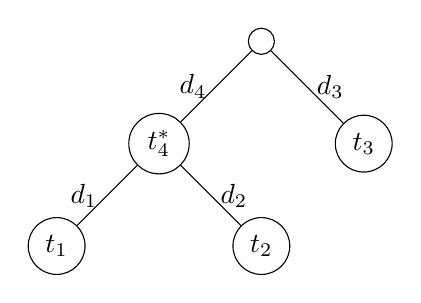
\begin{tikzpicture}[scale=1.3]
				\path (-2, -2) node[draw, circle] (n1){$t_1$}
				(0, -2) node[draw, circle] (n2){$t_2$}
				(1, -1) node[draw, circle] (n3){$t_3$}
				(-1, -1) node[draw, circle] (n4){$t_4^*$}
				(0, 0) node[draw, circle] (n5){};
				
				\draw (n1) -- node[anchor=east] {$d_1$} (n4) -- node[anchor=east] {$d_4$} (n5) -- node[anchor=west] {$d_3$} (n3)
				(n4) -- node[anchor=west] {$d_2$} (n2);				
			\end{tikzpicture}
			\subcaption{}
			\end{subfigure}
			\begin{subfigure}{.3\textwidth}
			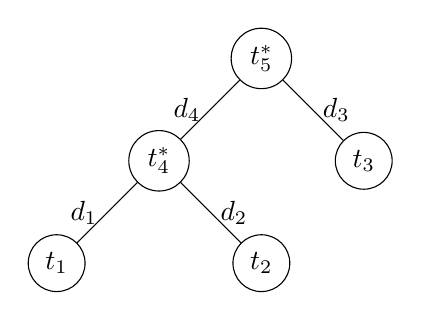
\begin{tikzpicture}[scale=1.3]
				\path (-2, -2) node[draw, circle] (n1){$t_1$}
				(0, -2) node[draw, circle] (n2){$t_2$}
				(1, -1) node[draw, circle] (n3){$t_3$}
				(-1, -1) node[draw, circle] (n4){$t_4^*$}
				(0, 0) node[draw, circle] (n5){$t_5^*$};
				
				\draw (n1) -- node[anchor=east] {$d_1$} (n4) -- node[anchor=east] {$d_4$} (n5) -- node[anchor=west] {$d_3$} (n3)
				(n4) -- node[anchor=west] {$d_2$} (n2);				
			\end{tikzpicture}
			\subcaption{}
			\end{subfigure}
			\caption{Initially the tree in (a) has edge lengths $d_1, \ldots, d_5$ and times on the tips, $t_1$, $t_2$, and $t_3$. In the first step, the algorithm processes internal nodes in the order of distance from the root. First $t_4^*$ is chosen (b) to maximize the product of likelihoods of the node's child edges using times, $t_1$ and $t_2$, and edge lengths, $d_1$ and $d_2$. Next $t_5^*$ is chosen (c) to maximize the product of likelihoods of the node's child edges using times, $t_3$ and $t_4^*$, and edge lengths, $d_3$ and $d_4$.
			\label{fig:init}}
		\end{figure}
		
		Then the algorithm runs sucessive steps now choosing the date to maximize the product of rthe likelihoods of all of a node's edges (See Figure \ref{fig:step}). The algorithm runs a specificied number of steps or until the difference in successive likelihoods of the tree is less than a specificed threshold.

		\begin{figure}[h]
			\centering
			\begin{subfigure}{.3\textwidth}
			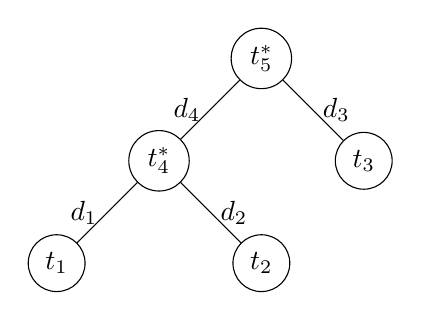
\begin{tikzpicture}[scale=1.3]
				\path (-2, -2) node[draw, circle] (n1){$t_1$}
				(0, -2) node[draw, circle] (n2){$t_2$}
				(1, -1) node[draw, circle] (n3){$t_3$}
				(-1, -1) node[draw, circle] (n4){$t_4^*$}
				(0, 0) node[draw, circle] (n5){$t_5^*$};
				
				\draw (n1) -- node[anchor=east] {$d_1$} (n4) -- node[anchor=east] {$d_4$} (n5) -- node[anchor=west] {$d_3$} (n3)
				(n4) -- node[anchor=west] {$d_2$} (n2);				
			\end{tikzpicture}
			\subcaption{}
			\end{subfigure}
			\begin{subfigure}{.3\textwidth}
			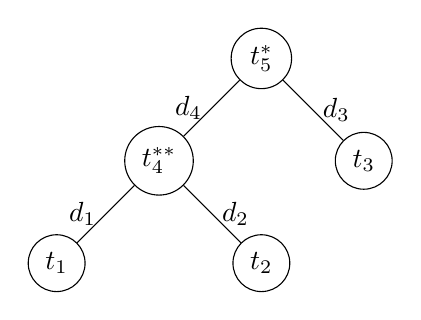
\begin{tikzpicture}[scale=1.3]
				\path (-2, -2) node[draw, circle] (n1){$t_1$}
				(0, -2) node[draw, circle] (n2){$t_2$}
				(1, -1) node[draw, circle] (n3){$t_3$}
				(-1, -1) node[draw, circle] (n4){$t_4^{**}$}
				(0, 0) node[draw, circle] (n5){$t_5^*$};
				
				\draw (n1) -- node[anchor=east] {$d_1$} (n4) -- node[anchor=east] {$d_4$} (n5) -- node[anchor=west] {$d_3$} (n3)
				(n4) -- node[anchor=west] {$d_2$} (n2);				
			\end{tikzpicture}
			\subcaption{}
			\end{subfigure}
			\begin{subfigure}{.3\textwidth}
			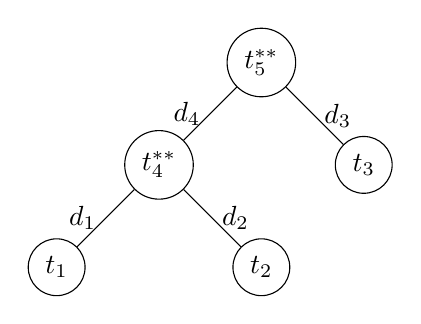
\begin{tikzpicture}[scale=1.3]
				\path (-2, -2) node[draw, circle] (n1){$t_1$}
				(0, -2) node[draw, circle] (n2){$t_2$}
				(1, -1) node[draw, circle] (n3){$t_3$}
				(-1, -1) node[draw, circle] (n4){$t_4^{**}$}
				(0, 0) node[draw, circle] (n5){$t_5^{**}$};
				
				\draw (n1) -- node[anchor=east] {$d_1$} (n4) -- node[anchor=east] {$d_4$} (n5) -- node[anchor=west] {$d_3$} (n3)
				(n4) -- node[anchor=west] {$d_2$} (n2);				
			\end{tikzpicture}
			\subcaption{}
			\end{subfigure}
			\caption{At the start, (a), of the second step of the algorithm the tree's internal nodes have times: $t_4^*$ and $t_5^*$.  Again, the algorithm processes internal nodes in the order of distance from the root. First $t_4^{**}$ is chosen (b) to maximize the product of likelihoods of the node's edges using times, $t_1$, $t_2$, and $t_5^*$, and edge lengths, $d_1$, $d_2$ and $d_4$. Next $t_5^{**}$ is chosen (c) to maximize the product of likelihoods of the node's child edges using times, $t_3$ and $t_4^{**}$, and edge lengths, $d_3$ and $d_4$.
			\label{fig:step}}
		\end{figure}	
	
	\section{Likelihood function}
		The likelihood of an assignment of dates, $\mathbf{t}$, to the nodes of a phylogenetic tree, $T$, is defined as the product of the likelihood of the edges:
		\[\mathcal{L}_T(\mathbf{t}) = \prod_{e \in E(T)}\mathcal{L}_e(\mathbf{t}_{p(e)} - \mathbf{t}_{c(e)}),\]
		where $p(e), c(e)$ are the parent and child nodes of the edge, $e$.
		The likelihood of an edge, $e$, is given by the gamma distribution:
		\[\mathcal{L}_e(t) = \operatorname{Gamma}(t; d(e) + 1, \mu) = \frac{{(d(e) + 1)}^{\mu}}{\Gamma(d(e) + 1)}t^{d(e)}e^{-\mu t},\]
		with $\mu$: the mutation rate and $d(e)$: the length of $e$.
		
		For efficiency, \code{node.dating}, uses the log likelihood instead of the likelihood to give:
		\[\log\mathcal{L}_e(t) = \mu\log d(e) - \log\Gamma(d(e) + 1) + d(e) \log t - \mu t,\]
		and the log likelihood of the tree is given by:
		\[\log\mathcal{L}_T(t) = \sum_{e \in E(T)} \left(\mu\log (d(e) + 1) - \log\Gamma(d(e) + 1) + d(e) \log (t_{p(e)} - t_{c(e)}) - \mu (t_{p(e)} - t_{c(e)})\right).\]
		
	\printbibliography{}
\end{document}